%%%%%%%%%%%%%%%%%%%%%%%%%%%%%%%%%%%%%%%%%%%%%%%%%%%%%%%%%%%%%%%%%%%%%%%%%%
%%
%%  Unified Author Submission Template for INFORMS Journals
%%  Based on official INFORMS templates (2024-2025)
%%  Modified by Jiheng Zhang @ UST
%%
%%%%%%%%%%%%%%%%%%%%%%%%%%%%%%%%%%%%%%%%%%%%%%%%%%%%%%%%%%%%%%%%%%%%%%%%%%
%
% Journal options - uncomment ONE:
%   mnsc - Management Science
%   opre - Operations Research
%   moor - Mathematics of Operations Research
%   msom - Manufacturing & Service Operations Management
%   isre - Information Systems Research
%   mksc - Marketing Science
%   orsc - Organization Science
%   trsc - Transportation Science
%   deca - Decision Analysis
%   ijoc - INFORMS Journal on Computing
%   stsy - Stochastic Systems
%   serv - Service Science
%
% Review options:
%   dblanonrev - Double Anonymous Review (blind)
%   sglanonrev - Single Anonymous Review (non-blind)
%
\documentclass[opre,sglanonrev]{informs4}
% \documentclass[mnsc,dblanonrev]{informs4}
% \documentclass[moor,sglanonrev]{informs4}

% Bibliography style (informs2014.bst required in same folder)
\bibliographystyle{informs2014}

% Additional packages (supplements what informs4.cls provides)
%% ==========================================================================
%% preamble.tex - Core LaTeX packages for academic papers
%% ==========================================================================
%% Include with: %% ==========================================================================
%% preamble.tex - Core LaTeX packages for academic papers
%% ==========================================================================
%% Include with: %% ==========================================================================
%% preamble.tex - Core LaTeX packages for academic papers
%% ==========================================================================
%% Include with: \input{preamble.tex}
%% For TikZ figures, also include: \input{tikz/setup.tex}
%% ==========================================================================

%%% Core math and graphics
\usepackage{amsmath,amssymb,amsfonts}
\usepackage{amsthm}             % theorem environments (proof, etc.)
\usepackage{mathtools}          % extends amsmath
\usepackage{mathrsfs}           % \mathscr for script fonts
\usepackage{bm}                 % bold math symbols
\usepackage{graphicx}
\usepackage{xcolor}             % color support

%%% Typography
\usepackage{microtype}          % better typography (kerning, spacing)
\usepackage[english]{babel}     % hyphenation patterns
\usepackage{setspace}           % line spacing (\onehalfspacing, \doublespacing)

%%% Tables
\usepackage{booktabs}           % professional tables (\toprule, \midrule, \bottomrule)
\usepackage{multirow}           % multi-row cells in tables
\usepackage{array}              % extended column definitions

%%% Figures
\usepackage{caption}
\captionsetup{
  justification=raggedright,
  singlelinecheck=false
}
\usepackage{subcaption}         % subfigures (\begin{subfigure})

%%% Algorithms (comment out if not needed)
\usepackage[ruled,vlined]{algorithm2e}

%%% Document structure
\usepackage{subfiles}           % multi-file documents
\usepackage[toc,page,title,titletoc]{appendix}

%%% Hyperlinks (load near end - redefines many commands)
\PassOptionsToPackage{hyphens}{url}  % allow URL line breaks at hyphens
% Define custom link colors (dark blue scheme, print-friendly)
\definecolor{linkblue}{rgb}{0.0, 0.0, 0.55}      % dark navy for internal refs
\definecolor{citeblue}{rgb}{0.0, 0.0, 0.55}      % dark navy for citations
\definecolor{urlblue}{rgb}{0.0, 0.25, 0.55}      % subtle teal for URLs
\usepackage{hyperref}
\hypersetup{
  colorlinks=true,
  linkcolor=linkblue,
  citecolor=citeblue,
  urlcolor=urlblue,
  plainpages=false,
  hypertexnames=false
}
\usepackage{bookmark}           % better PDF bookmarks (must follow hyperref)

%% For TikZ figures, also include: %% ==========================================================================
%% tikz/setup.tex - TikZ and pgfplots packages
%% ==========================================================================
%% Include with: \input{tikz/setup.tex}
%% Remove this input if your paper doesn't use TikZ figures.
%% ==========================================================================

%%% TikZ and plotting
\usepackage{tikz}
\usetikzlibrary{shapes,shapes.arrows,arrows,arrows.meta,positioning,calc,patterns,decorations.pathreplacing,topaths,automata}
\usepackage{pgfplots}
\usepgfplotslibrary{groupplots,dateplot}
\usepackage{pgfplotstable}
\pgfplotsset{compat=1.18}

%%% Add more TikZ libraries as needed:
% \usetikzlibrary{backgrounds}
% \usetikzlibrary{fit}
% \usetikzlibrary{matrix}
% \usetikzlibrary{chains}

%% ==========================================================================

%%% Core math and graphics
\usepackage{amsmath,amssymb,amsfonts}
\usepackage{amsthm}             % theorem environments (proof, etc.)
\usepackage{mathtools}          % extends amsmath
\usepackage{mathrsfs}           % \mathscr for script fonts
\usepackage{bm}                 % bold math symbols
\usepackage{graphicx}
\usepackage{xcolor}             % color support

%%% Typography
\usepackage{microtype}          % better typography (kerning, spacing)
\usepackage[english]{babel}     % hyphenation patterns
\usepackage{setspace}           % line spacing (\onehalfspacing, \doublespacing)

%%% Tables
\usepackage{booktabs}           % professional tables (\toprule, \midrule, \bottomrule)
\usepackage{multirow}           % multi-row cells in tables
\usepackage{array}              % extended column definitions

%%% Figures
\usepackage{caption}
\captionsetup{
  justification=raggedright,
  singlelinecheck=false
}
\usepackage{subcaption}         % subfigures (\begin{subfigure})

%%% Algorithms (comment out if not needed)
\usepackage[ruled,vlined]{algorithm2e}

%%% Document structure
\usepackage{subfiles}           % multi-file documents
\usepackage[toc,page,title,titletoc]{appendix}

%%% Hyperlinks (load near end - redefines many commands)
\PassOptionsToPackage{hyphens}{url}  % allow URL line breaks at hyphens
% Define custom link colors (dark blue scheme, print-friendly)
\definecolor{linkblue}{rgb}{0.0, 0.0, 0.55}      % dark navy for internal refs
\definecolor{citeblue}{rgb}{0.0, 0.0, 0.55}      % dark navy for citations
\definecolor{urlblue}{rgb}{0.0, 0.25, 0.55}      % subtle teal for URLs
\usepackage{hyperref}
\hypersetup{
  colorlinks=true,
  linkcolor=linkblue,
  citecolor=citeblue,
  urlcolor=urlblue,
  plainpages=false,
  hypertexnames=false
}
\usepackage{bookmark}           % better PDF bookmarks (must follow hyperref)

%% For TikZ figures, also include: %% ==========================================================================
%% tikz/setup.tex - TikZ and pgfplots packages
%% ==========================================================================
%% Include with: %% ==========================================================================
%% tikz/setup.tex - TikZ and pgfplots packages
%% ==========================================================================
%% Include with: \input{tikz/setup.tex}
%% Remove this input if your paper doesn't use TikZ figures.
%% ==========================================================================

%%% TikZ and plotting
\usepackage{tikz}
\usetikzlibrary{shapes,shapes.arrows,arrows,arrows.meta,positioning,calc,patterns,decorations.pathreplacing,topaths,automata}
\usepackage{pgfplots}
\usepgfplotslibrary{groupplots,dateplot}
\usepackage{pgfplotstable}
\pgfplotsset{compat=1.18}

%%% Add more TikZ libraries as needed:
% \usetikzlibrary{backgrounds}
% \usetikzlibrary{fit}
% \usetikzlibrary{matrix}
% \usetikzlibrary{chains}

%% Remove this input if your paper doesn't use TikZ figures.
%% ==========================================================================

%%% TikZ and plotting
\usepackage{tikz}
\usetikzlibrary{shapes,shapes.arrows,arrows,arrows.meta,positioning,calc,patterns,decorations.pathreplacing,topaths,automata}
\usepackage{pgfplots}
\usepgfplotslibrary{groupplots,dateplot}
\usepackage{pgfplotstable}
\pgfplotsset{compat=1.18}

%%% Add more TikZ libraries as needed:
% \usetikzlibrary{backgrounds}
% \usetikzlibrary{fit}
% \usetikzlibrary{matrix}
% \usetikzlibrary{chains}

%% ==========================================================================

%%% Core math and graphics
\usepackage{amsmath,amssymb,amsfonts}
\usepackage{amsthm}             % theorem environments (proof, etc.)
\usepackage{mathtools}          % extends amsmath
\usepackage{mathrsfs}           % \mathscr for script fonts
\usepackage{bm}                 % bold math symbols
\usepackage{graphicx}
\usepackage{xcolor}             % color support

%%% Typography
\usepackage{microtype}          % better typography (kerning, spacing)
\usepackage[english]{babel}     % hyphenation patterns
\usepackage{setspace}           % line spacing (\onehalfspacing, \doublespacing)

%%% Tables
\usepackage{booktabs}           % professional tables (\toprule, \midrule, \bottomrule)
\usepackage{multirow}           % multi-row cells in tables
\usepackage{array}              % extended column definitions

%%% Figures
\usepackage{caption}
\captionsetup{
  justification=raggedright,
  singlelinecheck=false
}
\usepackage{subcaption}         % subfigures (\begin{subfigure})

%%% Algorithms (comment out if not needed)
\usepackage[ruled,vlined]{algorithm2e}

%%% Document structure
\usepackage{subfiles}           % multi-file documents
\usepackage[toc,page,title,titletoc]{appendix}

%%% Hyperlinks (load near end - redefines many commands)
\PassOptionsToPackage{hyphens}{url}  % allow URL line breaks at hyphens
% Define custom link colors (dark blue scheme, print-friendly)
\definecolor{linkblue}{rgb}{0.0, 0.0, 0.55}      % dark navy for internal refs
\definecolor{citeblue}{rgb}{0.0, 0.0, 0.55}      % dark navy for citations
\definecolor{urlblue}{rgb}{0.0, 0.25, 0.55}      % subtle teal for URLs
\usepackage{hyperref}
\hypersetup{
  colorlinks=true,
  linkcolor=linkblue,
  citecolor=citeblue,
  urlcolor=urlblue,
  plainpages=false,
  hypertexnames=false
}
\usepackage{bookmark}           % better PDF bookmarks (must follow hyperref)


% TikZ packages - remove if not using TikZ figures
%% ==========================================================================
%% tikz/setup.tex - TikZ and pgfplots packages
%% ==========================================================================
%% Include with: %% ==========================================================================
%% tikz/setup.tex - TikZ and pgfplots packages
%% ==========================================================================
%% Include with: %% ==========================================================================
%% tikz/setup.tex - TikZ and pgfplots packages
%% ==========================================================================
%% Include with: \input{tikz/setup.tex}
%% Remove this input if your paper doesn't use TikZ figures.
%% ==========================================================================

%%% TikZ and plotting
\usepackage{tikz}
\usetikzlibrary{shapes,shapes.arrows,arrows,arrows.meta,positioning,calc,patterns,decorations.pathreplacing,topaths,automata}
\usepackage{pgfplots}
\usepgfplotslibrary{groupplots,dateplot}
\usepackage{pgfplotstable}
\pgfplotsset{compat=1.18}

%%% Add more TikZ libraries as needed:
% \usetikzlibrary{backgrounds}
% \usetikzlibrary{fit}
% \usetikzlibrary{matrix}
% \usetikzlibrary{chains}

%% Remove this input if your paper doesn't use TikZ figures.
%% ==========================================================================

%%% TikZ and plotting
\usepackage{tikz}
\usetikzlibrary{shapes,shapes.arrows,arrows,arrows.meta,positioning,calc,patterns,decorations.pathreplacing,topaths,automata}
\usepackage{pgfplots}
\usepgfplotslibrary{groupplots,dateplot}
\usepackage{pgfplotstable}
\pgfplotsset{compat=1.18}

%%% Add more TikZ libraries as needed:
% \usetikzlibrary{backgrounds}
% \usetikzlibrary{fit}
% \usetikzlibrary{matrix}
% \usetikzlibrary{chains}

%% Remove this input if your paper doesn't use TikZ figures.
%% ==========================================================================

%%% TikZ and plotting
\usepackage{tikz}
\usetikzlibrary{shapes,shapes.arrows,arrows,arrows.meta,positioning,calc,patterns,decorations.pathreplacing,topaths,automata}
\usepackage{pgfplots}
\usepgfplotslibrary{groupplots,dateplot}
\usepackage{pgfplotstable}
\pgfplotsset{compat=1.18}

%%% Add more TikZ libraries as needed:
% \usetikzlibrary{backgrounds}
% \usetikzlibrary{fit}
% \usetikzlibrary{matrix}
% \usetikzlibrary{chains}


% Line spacing (default: 1.5 spacing with 11pt font)
\OneAndAHalfSpacedXI
%\OneAndAHalfSpacedXII  % 1.5 spacing with 12pt font
%\DoubleSpacedXI        % Double spacing with 11pt font
%\DoubleSpacedXII       % Double spacing with 12pt font

% Equation numbering (uncomment one)
\EquationsNumberedThrough    % Default: (1), (2), ...
%\EquationsNumberedBySection % (1.1), (1.2), ...

% Theorem numbering (uncomment one)
\TheoremsNumberedThrough     % Preferred (Theorem 1, Lemma 1, Theorem 2)
%\TheoremsNumberedByChapter  % (Theorem 1.1, Lemma 1.1, Theorem 1.2)
\ECRepeatTheorems

% For revisions, input manuscript number with suffix ".Rx"
% \MANUSCRIPTNO{OPRE-0001-2024.00}

%%%%%%%%%%%%%%%%
\begin{document}
%%%%%%%%%%%%%%%%

% Running heads (optional for submission)
% \RUNAUTHOR{Zhang}
% \RUNTITLE{Short Title}

% Full title
\TITLE{An Important and Impactful Paper}

% Authors and affiliations
\ARTICLEAUTHORS{%
\AUTHOR{Richard Feynman, Albert Einstein, and Leonhard Euler}
\AFF{The Hong Kong University of Science and Technology, Clear~Water~Bay, Hong Kong S.A.R., China\\
\EMAIL{\{feyman, einstein, euler\}@ust.hk}}
}

\ABSTRACT{
% big background
Stochastic control in multi-class queueing networks has been extensively studied primarily focusing on minimizing operational costs (e.g., waiting, abandonment).
% what is novel
However, in many real-world applications, the system operator must balance the trade-off between waiting costs and maximizing immediate rewards when assigning customers to service units.
}

% \FUNDING{This research was supported by [grant number, funding agency].}

\KEYWORDS{Stochastic control, Queueing network, Uncertainty, Online learning, Optimization}

% \HISTORY{Received: Month DD, YYYY; Accepted: Month DD, YYYY}

\maketitle
%%%%%%%%%%%%%%%%%%%%%%%%%%%%%%%%%%%%%%%%%%%%%%%%%%%%%%%%%%%%%%%%%%%%%%

\section{Introduction}

\cite{Erlang1948,Dantzig1955,Dynkin1956,Bellman1957DP,Little1961,Skorokhod1961,McKean1965,Iglehart1965}

\section{Model}

\begin{figure}[htbp]
  \centering
  \begin{tikzpicture}[scale=1.5]
    \label{fig:N-model-rework}
    % Draw axes
    \draw [<->,thick] (0,5) node (yaxis) [above] {$x_2$}
        |- (5,0) node (xaxis) [right] {$x_1$};
    % Draw two intersecting lines
    \draw (0,0) coordinate (a_1) -- (1.6,2) coordinate (a_2);
    \draw (1.6,2) coordinate (b_1) -- (1.6,4.75) coordinate (b_2);
    \draw[dashed] (0,4.88) -- (2.7111,0);
    \node at (3.4,0.4) {$s_2(\bar W(t))=K_2$};

    \coordinate (c) at (intersection of a_1--a_2 and b_1--b_2);
    % Draw lines indicating intersection with y and x axis. Here we use
    % the perpendicular coordinate system
    \draw[dashed] (yaxis |- c) node[left] {$K_2$}
        -| (xaxis -| c) node[below] {$\frac{\mu_2K_2}{\mu_1}$};
    \draw[dashed] (2.2, 0.05) -- (2.2,0) node[below] {$K_1$};
    % Draw a dot to indicate intersection point

    \coordinate (a) at (2.4,0.8);
    \fill[red] (a) circle (1pt);
    \draw[blue] (a) -- (1.6,0.8);

    \coordinate (b) at (1.94,0.9);
    \fill[red] (b) circle (1pt);
    \draw[blue] (b) -- (1.44,1.8);
\end{tikzpicture}
  \caption{Sample x-y plot}
  \label{fig:x-y}
\end{figure}

\section{Conclusion}

\begin{figure}[htbp]
  \centering
  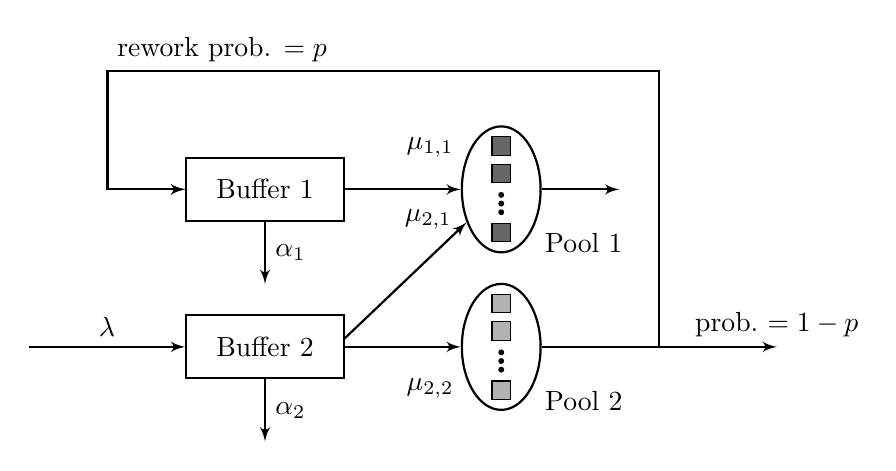
\begin{tikzpicture}[auto, >=latex']
    \everymath{\displaystyle}
    \tikzstyle{every picture}+=[remember picture]

    \tikzstyle{coor-format} = [coordinate]
    \tikzstyle{b-format} = [draw=black, thick,
                            minimum height=0.8cm, minimum width=2cm]
    \tikzstyle{s1-format} = [rectangle, draw=black, fill=black!60]
    \tikzstyle{s2-format} = [rectangle, draw=black, fill=black!30]
    \tikzstyle{p-format} = [ellipse, draw=black, thick,
                            minimum height=1.6cm, minimum width=1cm]

    \node [coor-format] (In1) {};
    \node [b-format, right of=In1, node distance=2cm] (Buf1) {Buffer 1};
    \draw [draw,->, thick] (In1) -- (Buf1);

    \node [coor-format, below of=Buf1, node distance=1.2cm] (Abd1) {};
    \draw [draw,->, thick] (Buf1) -- node {$\alpha_1$} (Abd1);

    \node [p-format, right of=Buf1, node distance=3cm, label=-45:Pool 1,
           label=150:{$\mu_{1,1}$}, label=-165:{$\mu_{2,1}$}] (Pool1) {};
    \draw [draw,->, thick] (Buf1) -- (Pool1);

    \node [coor-format, right of=Pool1, node distance=1.5cm] (Out1) {};
    \draw [draw,->, thick] (Pool1) -- (Out1);

    \node [coor-format,below of = In1, node distance = 2cm] (In2) {};
    \node [b-format, right of=In2, node distance=2cm] (Buf2) {Buffer 2};
    \draw [draw,->, thick] (In2)+(-1cm,0) --node {$\lambda$} (Buf2);

    \node [p-format, right of=Buf2, node distance=3cm,
           label=-45:Pool 2,label=-150:$\mu_{2,2}$] (Pool2) {};
    \draw [draw,->, thick] (Buf2) -- (Pool2);
    \draw [draw,->, thick] (Buf2.east)+(-0.01cm,0.1cm) -- (Pool1);

    \node [coor-format, below of=Buf2, node distance=1.2cm] (Abd2) {};
    \draw [draw,->, thick] (Buf2) -- node {$\alpha_2$} (Abd2);

    \node [coor-format, right of=Pool2, node distance=3.5cm,
    label=90:{prob.\ $=1-p$}] (Out2) {};
    \draw [draw,->, thick] (Pool2) -- (Out2);

    \node [coor-format, above of = In1,
           node distance=1.5cm, label=45:rework prob. {$=p$}](upper-left){};
    \path [draw, -, thick] (Out2)+(-1.5cm,0) |- (upper-left);

    \draw [draw, ->, thick] (upper-left)+(0,0.014cm) |- (Buf1);

    \node at (5cm,0.55cm) [s1-format]{};
    \node at (5cm,0.2cm) [s1-format]{};
    \draw [draw=black, fill=black]
           (5cm,-0.07cm) circle (0.03cm);
    \draw [draw=black, fill=black]
           (5cm,-0.18cm) circle (0.03cm);
    \draw [draw=black, fill=black]
           (5cm,-0.29cm) circle (0.03cm);
    \node at (5cm,-0.55cm) [s1-format]{};

    \node at (5cm,0.55cm-2cm) [s2-format]{};
    \node at (5cm,0.2cm-2cm) [s2-format]{};
    \draw [draw=black, fill=black]
           (5cm,-0.07cm-2cm) circle (0.03cm);
    \draw [draw=black, fill=black]
           (5cm,-0.18cm-2cm) circle (0.03cm);
    \draw [draw=black, fill=black]
           (5cm,-0.29cm-2cm) circle (0.03cm);
    \node at (5cm,-0.55cm-2cm) [s2-format]{};
\end{tikzpicture}

  \caption{A schematic Model of Outsourcing with rework}
  \label{fig:N-model-rework}
\end{figure}

% Code and Data Disclosure (required for OPRE, likely other journals)
% \section{Code and Data Disclosure}
% The code and data to support the numerical experiments in this paper can be found at [URL].

% Acknowledgments
% \ACKNOWLEDGMENT{We thank...}

\bibliography{ref}

%%%%%%%%%%%%%%%%%%%%%%%%%%%%%%%%%%%%%%%%%%%%%%%%%%%%%%%%%%%%%%%%%%%%%%
% Electronic Companion (EC) starts here
%%%%%%%%%%%%%%%%%%%%%%%%%%%%%%%%%%%%%%%%%%%%%%%%%%%%%%%%%%%%%%%%%%%%%%

\ECSwitch
\ECHead{Proofs}

\section{Proof of Results}

\subsection{Proof of Lemma}

\begin{lemma}
    \label{lem:A1}
    As long as $t>8 \frac{d \log 9 +\log (T/\alpha)}{p_{*}^2}$, the following lower bound
\end{lemma}

\begin{proof}{Proof of Lemma~\ref{lem:A1}}
\Halmos
\end{proof}

%%%%%%%%%%%%%%%%%
\end{document}
%%%%%%%%%%%%%%%%%
